O desenvolvimento do projeto NitrusLeaf foi estruturado em etapas organizadas de forma sequencial e iterativa, com base em princípios de desenvolvimento ágil, visando flexibilidade e adaptação ao longo do processo. O método adotado busca garantir a integração eficiente entre as etapas de análise, implementação e validação dos resultados, assegurando a qualidade e a aplicabilidade da solução desenvolvida.

A Figura \ref{fig:fluxograma} apresenta o fluxograma geral do processo metodológico, descrevendo a sequência lógica das atividades realizadas, desde a captura das imagens até o registro final dos diagnósticos no sistema.

\begin{figure}[H]
    \centering
    \caption{Fluxograma do processo de classificação das folhas de mexerica}
    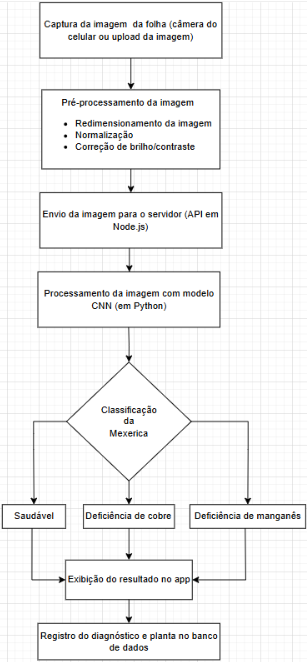
\includegraphics[width=0.6\linewidth]{Illustrations/fluxograma.png}
    \label{fig:fluxograma}
    \SourceOrNote{Fonte: autoria própria (2025)}
\end{figure}

A seguir, descrevem-se detalhadamente as etapas que compõem o processo metodológico representado no fluxograma:

\begin{enumerate}
\item \textbf{Coleta de Requisitos e Planejamento do Sistema}

Nesta etapa inicial, foram levantados os requisitos funcionais e não funcionais do sistema, definindo-se as principais funcionalidades e fluxos de interação. Para o planejamento da interface e prototipagem, utilizou-se o Figma, devido à sua facilidade de colaboração e à capacidade de criar protótipos interativos de baixa e alta fidelidade. Essa fase também incluiu a elaboração de diagramas UML para a representação da estrutura do sistema e análise SWOT para identificar forças, fraquezas, oportunidades e ameaças, garantindo uma visão ampla do projeto.

\item \textbf{Captura e Pré-processamento das Imagens}

O processo tem início com a captura de imagens de folhas de mexerica por meio da câmera do celular ou upload de imagens previamente armazenadas. As imagens passam por etapas de pré-processamento, incluindo redimensionamento, normalização e correção de brilho e contraste. Essas operações garantem a padronização dos dados visuais, fundamentais para o bom desempenho da CNN durante a classificação.

\item \textbf{Envio e Processamento das Imagens}

Após o pré-processamento, as imagens são enviadas para o servidor por meio de uma API desenvolvida em Node.js. No servidor, o modelo de IA implementado em Python realiza o processamento utilizando redes neurais convolucionais (CNNs) treinadas previamente com imagens rotuladas de folhas saudáveis e com deficiências de cobre e manganês. Essa etapa representa o núcleo analítico do sistema, onde ocorre a classificação automática das imagens.

\item \textbf{Classificação e Exibição dos Resultados}

O modelo realiza a classificação das folhas em três categorias: saudável, deficiência de cobre ou deficiência de manganês. O resultado é exibido no aplicativo em tempo real, fornecendo ao usuário um diagnóstico rápido e acessível. Essa abordagem visa permitir a identificação imediata de deficiências no campo, reduzindo o tempo entre o diagnóstico e a tomada de decisão pelo agricultor.

\item \textbf{Registro e Armazenamento dos Diagnósticos}

Os diagnósticos gerados são armazenados no banco de dados, associados ao registro da planta e ao talhão correspondente. Essa funcionalidade possibilita o acompanhamento histórico do estado nutricional das plantas, facilitando análises posteriores e o monitoramento contínuo das condições do cultivo.

\item \textbf{Treinamento e Avaliação do Modelo}

O treinamento do modelo de IA foi realizado a partir de um conjunto de imagens rotuladas, aplicando técnicas de \textit{data augmentation} para aumentar a diversidade visual do conjunto. Foram utilizadas métricas de desempenho como acurácia, precisão e F1-score para validar o modelo. A metodologia de avaliação segue princípios semelhantes aos empregados por \textcite{Tran2019}, que demonstraram a importância da validação cruzada e da comparação de arquiteturas para garantir resultados consistentes e confiáveis.

\item \textbf{Ferramentas Utilizadas}

Para a implementação do sistema, foram empregadas diferentes ferramentas tecnológicas. O front-end foi desenvolvido com React e Next.js, oferecendo desempenho otimizado e boa organização estrutural. O back-end foi construído em Node.js, responsável pela integração com o banco de dados e a comunicação com o modelo de IA. O armazenamento de dados foi realizado com MySQL, escolhido pela robustez e ampla compatibilidade. O módulo de visão computacional foi desenvolvido em Python, pela facilidade de integração com bibliotecas voltadas à IA, como TensorFlow e Keras.
\end{enumerate}
